\documentclass[aspectratio=169,10pt]{beamer}
\usetheme{Madrid}
\setbeamertemplate{navigation symbols}{}
\usepackage{amsmath}
\usepackage{amssymb}
\usepackage{array}
\usepackage{booktabs}
\usepackage{graphicx}
\graphicspath{{analysis-4-1-agent-taxonomy/figures/}{analysis-4-2-family-separability/figures/}{analysis-4-3-rho-beta-identifiability/figures/}{analysis-4-4-local-heuristic-equivalence/figures/}{analysis-4-5-query-and-belief-design/figures/}{analysis-4-6-kl-visualisation-standard/figures/}{analysis-4-7-beyond-map-coloring/figures/}}

\title{Analysis 4 Summary}
\subtitle{Beyond $\rho$: completed work from Analyses 4-1 to 4-7}
\author{}
\date{\today}

\begin{document}

\begin{frame}
\titlepage
\end{frame}

\begin{frame}{What was completed}
\small
\begin{itemize}
    \item Analysis 4 is now complete as a coherent series, with shared code in \texttt{common/analysis4\_common.py}.
    \item Deliverables produced in this pass: 7 compiled reports, 16 figure PDFs, and 25 data outputs.
    \item The sub-analysis reports, README files, figures, and the slide deck are aligned to the same final version of the results.
\end{itemize}

\medskip
\scriptsize
\begin{tabular}{p{0.75cm}p{4.15cm}p{6.25cm}}
\toprule
ID & Focus & Main conclusion carried forward \\
\midrule
4-1 & Agent taxonomy & Retain six families; absorb the pure local log-evidence heuristic into $M_0$. \\
4-2 & Family separability & Current rooted library already separates structure rewrites strongly; exact vs.\ attenuation is much weaker. \\
4-3 & $\rho$ vs.\ $\beta$ identifiability & Joint modelling is needed unless analyses are restricted to a targeted diagnostic panel. \\
4-4 & Heuristic equivalence & The pure heuristic is exactly $M_0$ under the standard readout. \\
4-5 & Query plus belief design & Choose-node-then-report-belief is the cleanest richer behavioural extension. \\
4-6 & Visual standard & Future family comparisons now have a mandatory default figure suite. \\
4-7 & Beyond map-colouring & Attractive graph labelling is the recommended next task domain. \\
\bottomrule
\end{tabular}
\end{frame}

\begin{frame}{4-1. Model space after taxonomy cleanup}
\begin{columns}[T]
\column{0.43\textwidth}
\small
\begin{itemize}
    \item Retained family set:
    \[
    M_{\mathrm{exact}},\;
    M_0,\;
    M_{\rho},\;
    M_{\rho,\beta},\;
    M_{\mathrm{star}},\;
    M_{\mathrm{cluster}}.
    \]
    \item The central conceptual result is negative: the pure local log-evidence heuristic is not a seventh family.
    \item Under exponentiate-and-normalise readout it is exactly $M_0$, so Analysis 4 focuses on genuinely distinct structural approximations.
\end{itemize}

\column{0.57\textwidth}
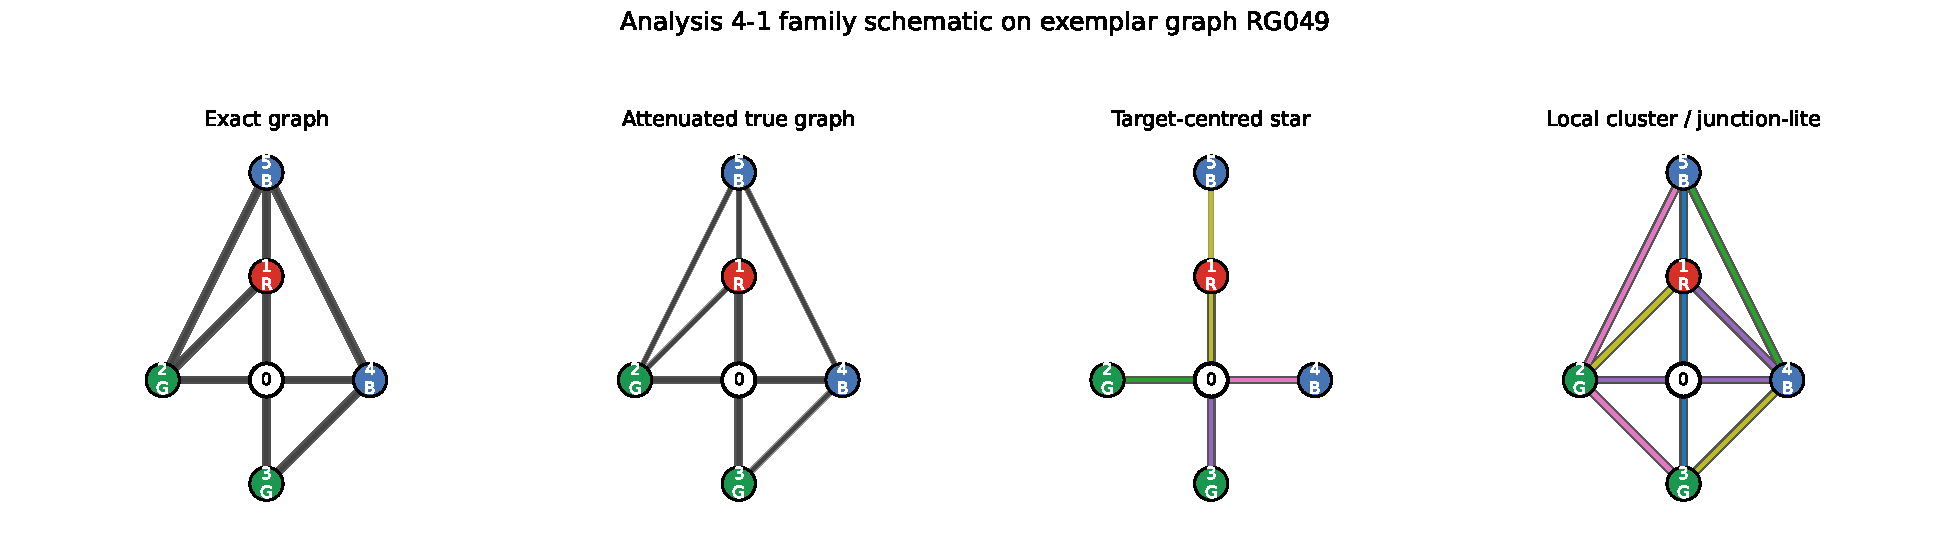
\includegraphics[width=\textwidth]{analysis-4-1_fig1_family_schematic.pdf}
\end{columns}
\end{frame}

\begin{frame}{4-2. Existing stimulus library already separates several families}
\begin{columns}[T]
\column{0.4\textwidth}
\small
\begin{itemize}
    \item Evaluated 600 rooted graph/evidence conditions.
    \item Strongest mean family contrast:
    \[
    \mathrm{JS}(M_{\mathrm{exact}}, M_{\mathrm{star}})=0.113605.
    \]
    \item Canonical attenuation remains close to exact inference:
    \[
    \mathrm{JS}(M_{\mathrm{exact}}, M_{\rho})=0.009751.
    \]
    \item Reduced high-value panel:
    RG119, RG112, RG121, RG114, RG036, RG100.
\end{itemize}

\column{0.6\textwidth}
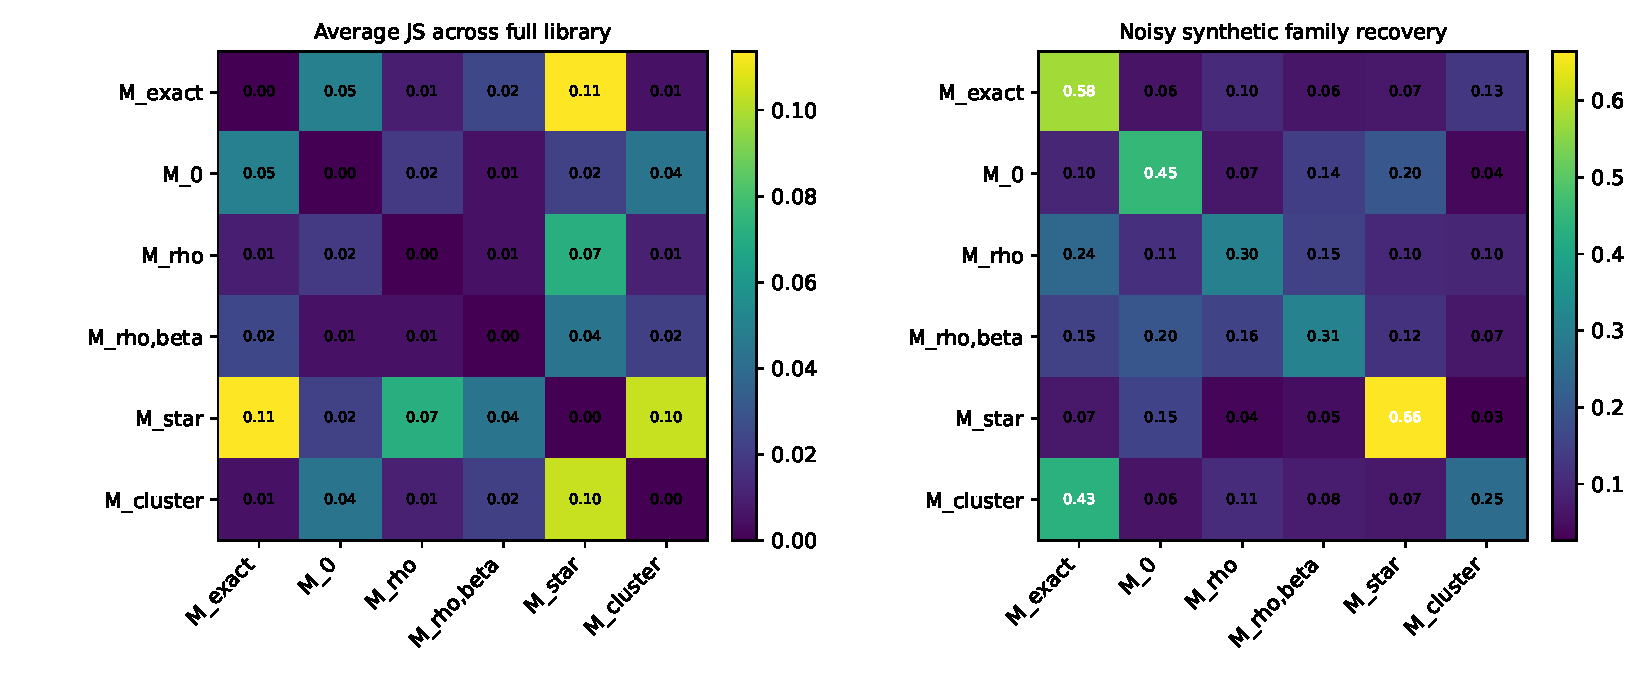
\includegraphics[width=\textwidth]{analysis-4-2_fig2_global_confusion.pdf}
\end{columns}
\end{frame}

\begin{frame}{4-3. $\rho$ and $\beta$ are identifiable in principle, but trade off under noise}
\begin{columns}[T]
\column{0.42\textwidth}
\small
\begin{itemize}
    \item Diagnostic recovery panel retained 8 high-value conditions.
    \item Noiseless exact-match rate: 1.0.
    \item Noisy exact-match rate: 0.3.
    \item Mean absolute error:
    \[
    |\hat{\rho}-\rho| = 0.136587,\quad
    |\hat{\beta}-\beta| = 0.584921.
    \]
    \item Recommendation: either fit $\rho$ and $\beta$ jointly, or restrict analyses to the diagnostic panel.
\end{itemize}

\column{0.58\textwidth}
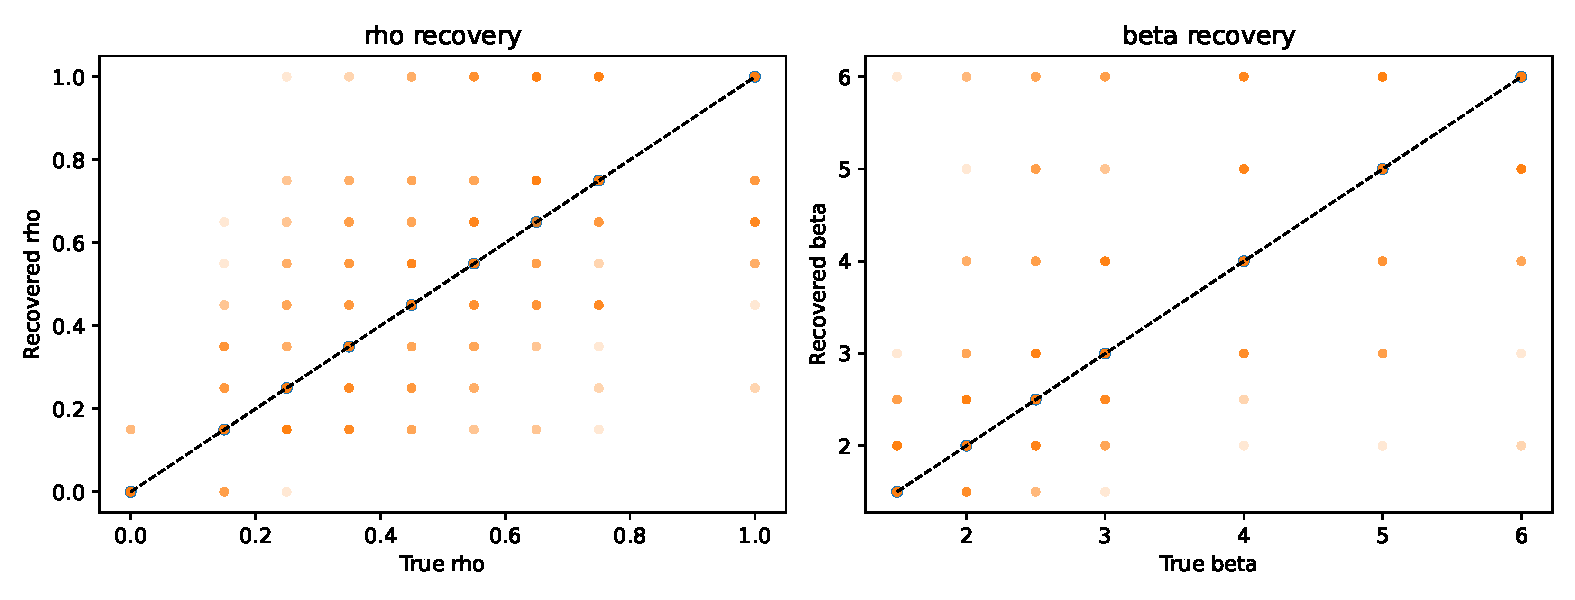
\includegraphics[width=\textwidth]{analysis-4-3_fig2_recovery.pdf}
\end{columns}
\end{frame}

\begin{frame}{4-4 and 4-5. Design consequences}
\begin{columns}[T]
\column{0.46\textwidth}
\small
\textbf{Heuristic equivalence (4-4)}
\begin{itemize}
    \item Maximum absolute difference between the pure heuristic and $M_0$: 0.0.
    \item Mean JS to $M_0$: 0.0.
    \item Only weighted or clipped variants produce genuinely new local baselines.
\end{itemize}

\medskip
\textbf{Richer behavioural design (4-5)}
\begin{itemize}
    \item Mean pairwise separation:
    \begin{itemize}
        \item belief-only: 0.003211
        \item selection-only: 0.030576
        \item combined: 0.054955
    \end{itemize}
    \item Recommendation: use fixed-evidence choose-node-then-report-belief as a targeted supplement, not yet a full replacement.
\end{itemize}

\column{0.54\textwidth}
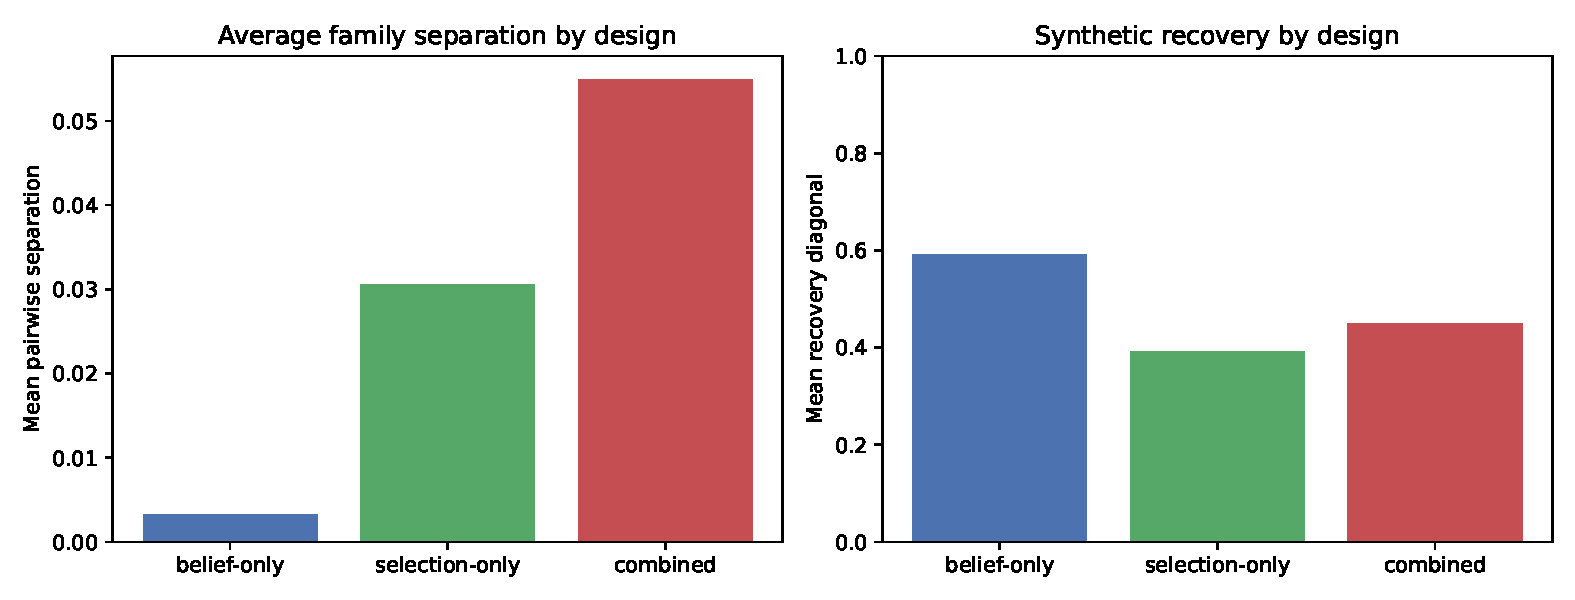
\includegraphics[width=\textwidth]{analysis-4-5_fig2_design_comparison.pdf}
\end{columns}
\end{frame}

\begin{frame}{4-6. A reusable visual reporting standard now exists}
\begin{columns}[T]
\column{0.44\textwidth}
\small
\begin{itemize}
    \item Mandatory figure suite:
    \begin{itemize}
        \item condition-specific family divergence heatmap
        \item target belief profile panel
        \item global family confusion summary
        \item rooted descriptor linkage summary
    \end{itemize}
    \item Worked example condition: RG112 at high evidence.
    \item D1/D2/D3 terminology is preserved so future analyses stay aligned with Analysis 3.
\end{itemize}

\column{0.56\textwidth}
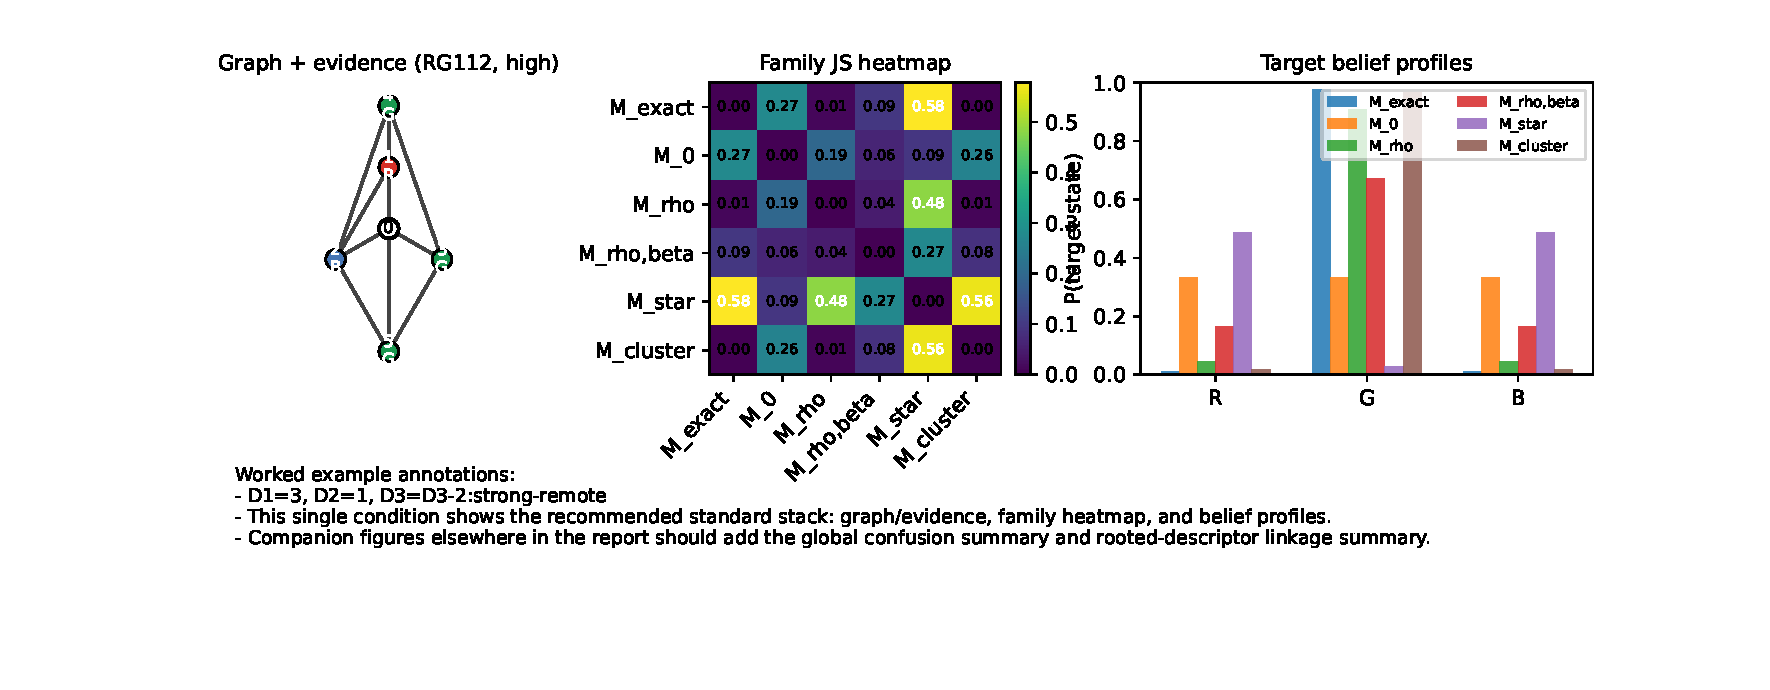
\includegraphics[width=\textwidth]{analysis-4-6_fig1_worked_example_panel.pdf}
\end{columns}
\end{frame}

\begin{frame}{4-7. Strategic extension beyond map-colouring}
\begin{columns}[T]
\column{0.43\textwidth}
\small
\begin{itemize}
    \item Current claims are strongest for repulsive local couplings.
    \item Recommended next domain: \texttt{attractive\_graph\_labelling}.
    \item Top weighted priorities:
    \begin{itemize}
        \item \texttt{attractive\_graph\_labelling}: 4.75
        \item \texttt{map\_colouring}: 4.1
        \item \texttt{social\_consensus}: 4.0
    \end{itemize}
    \item This is the cleanest way to test whether the same family taxonomy survives a reversal from repulsive to attractive local semantics.
\end{itemize}

\column{0.57\textwidth}
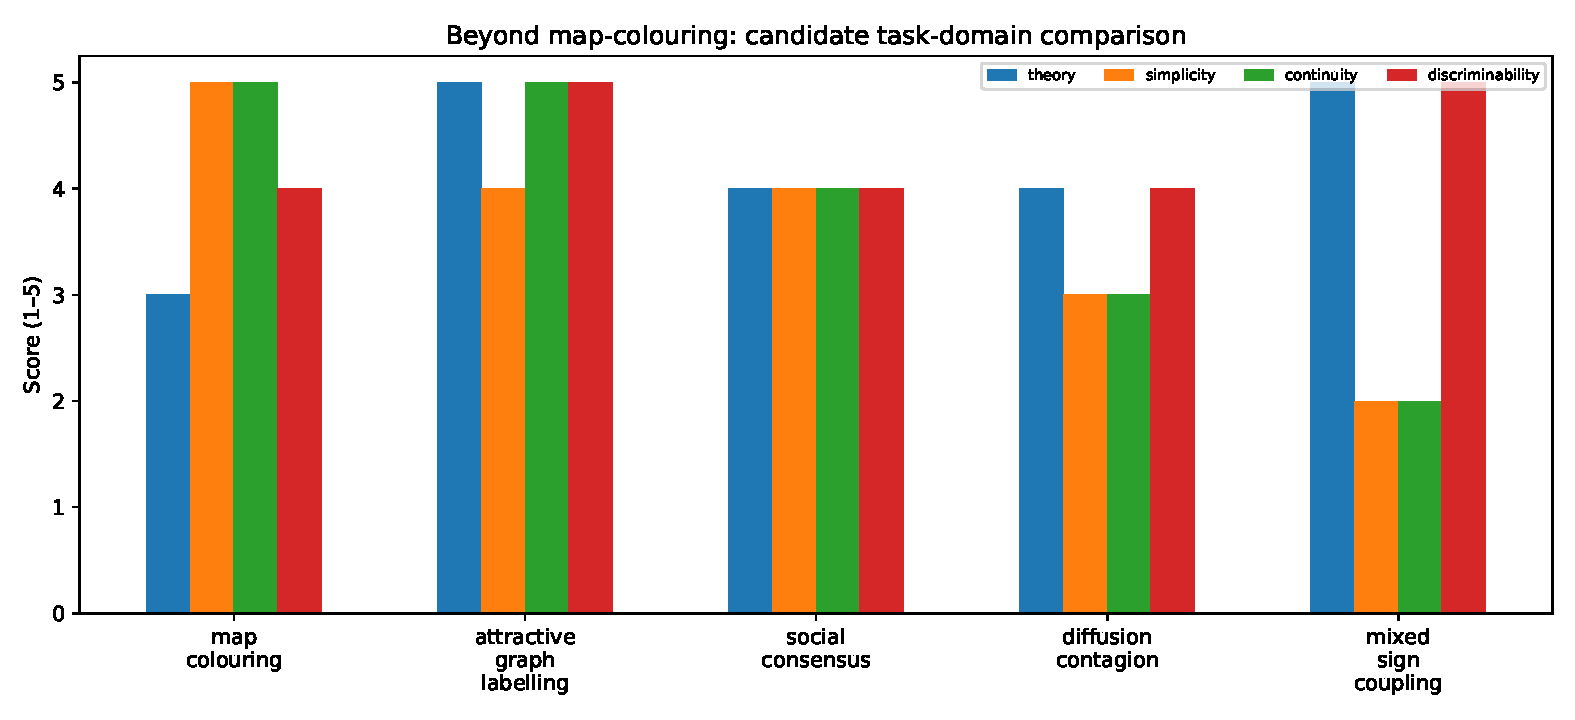
\includegraphics[width=\textwidth]{analysis-4-7_fig1_domain_comparison.pdf}
\end{columns}
\end{frame}

\begin{frame}{Bottom line}
\small
\begin{itemize}
    \item Analysis 4 expands the project from a single attenuation family to a structured model space with six simulation-ready families.
    \item The current rooted library is already very informative about structural rewrites, especially those involving $M_{\mathrm{star}}$ and $M_{\mathrm{cluster}}$.
    \item The main unresolved quantitative caution is the $\rho$--$\beta$ tradeoff, which is manageable but should not be ignored in downstream fitting.
    \item The pure local heuristic should not be carried forward as a separate core family.
    \item The strongest practical next steps are:
    \begin{enumerate}
        \item fit or test on the reduced diagnostic panels,
        \item add targeted choose-node-then-report-belief trials,
        \item extend the programme to attractive graph labelling.
    \end{enumerate}
\end{itemize}
\end{frame}

\end{document}
